\chapter{Greedy Algorithms}

\section{Introduction}

\term{Greedy algorithms} are a class of algorithms that make locally optimal choices at each step in order to find a global optimum. They are often used to solve optimization problems.

\begin{listu}
    \item \textbf{Goal:} find a solution $x$ maximizing or minimizing some objective function $f$.
    \item \textbf{Challenge:} space of possible solutions $x$ is too large to search exhaustively.
    \item \textbf{Insight:} $x$ is composed of several parts (e.g., $x$ is a set or a sequence).
    \item \textbf{Approach:} instead of computing $x$ directly,
    \begin{listu}
        \item Compute $x$ one part at a time.
        \item Select the next part ``greedily'' to get the most immediate ``benefit'', which needs to be defined carefully for each problem.
        \item Polynomial running time is typically guaranteed.
        \item Need to prove that this will always return an optimal solution despite having no global view of the problem.
    \end{listu}
\end{listu}

\section{Interval Scheduling}\label{sec:interval-scheduling}

\subsection{Problem Definition}

\begin{listu}
    \item Job $j$ starts at time $s_j$ and finishes at time $f_j$.
    \item Two jobs $i$ and $j$ are compatible if $[s_i, f_i)$ and $[s_j, f_j)$ do not overlap.
    \item \textbf{Goal:} find a maximum-size subset of mutually compatible jobs.
\end{listu}

\subsection{Greedy Algorithm}

The greedy algorithm for interval scheduling follows the template
\begin{listu}
    \item Consider jobs in some ``natural'' order.
    \item Take a job if it is compatible with the ones already taken.
\end{listu}

But, what is the ``natural'' order?
\begin{listu}
    \item \textbf{Earliest start time:} ascending order of $s_j$.
    \item \textbf{Earliest finish time:} ascending order of $f_j$.
    \item \textbf{Shortest interval:} ascending order of $f_j - s_j$.
    \item \textbf{Fewest conflicts:} ascending order of $c_j$, where $c_j$ is the number of remaining jobs that conflicts with job $j$.
\end{listu}

However, not all of these orders will yield the optimal solution. Below are some counterexamples.

{~~~}

\begin{minipage}[t]{0.55\linewidth}
    \begin{center} \tikzexternalenable \begin{tikzpicture}[baseline=(current bounding box.center)]
        \definecolor{lightGray}{gray}{0.7}
        \definecolor{darkGray}{gray}{0.5}

        \node[draw=none, fill=lightGray, minimum width=1cm, minimum height=0.25cm] at (0, 0) {};
        \node[draw=none, fill=lightGray, minimum width=1cm, minimum height=0.25cm] at (1.5, 0) {};
        \node[draw=none, fill=lightGray, minimum width=1cm, minimum height=0.25cm] at (3, 0) {};
        \node[draw=none, fill=lightGray, minimum width=1cm, minimum height=0.25cm] at (4.5, 0) {};

        \node[draw=none, fill=darkGray, minimum width=6.5cm, minimum height=0.25cm] at (2.25, -0.375) {};
    \end{tikzpicture} \tikzexternaldisable \end{center}
\end{minipage}
\begin{minipage}[t]{0.35\linewidth}
    \begin{center}
        Earliest Start Time
    \end{center}
\end{minipage}

{~~~}

{~~~}

\begin{minipage}[t]{0.55\linewidth}
    \begin{center} \tikzexternalenable \begin{tikzpicture}[baseline=(current bounding box.center)]
        \definecolor{lightGray}{gray}{0.7}
        \definecolor{darkGray}{gray}{0.5}

        \node[draw=none, fill=lightGray, minimum width=2cm, minimum height=0.25cm] at (0, 0) {};
        \node[draw=none, fill=lightGray, minimum width=2cm, minimum height=0.25cm] at (2.5, 0) {};

        \node[draw=none, fill=darkGray, minimum width=1.5cm, minimum height=0.25cm] at (1.25, -0.375) {};
    \end{tikzpicture} \tikzexternaldisable \end{center}
\end{minipage}
\begin{minipage}[t]{0.35\linewidth}
    \begin{center}
        Shortest Interval
    \end{center}
\end{minipage}

{~~~}

{~~~}

\begin{minipage}[t]{0.55\linewidth}
    \begin{center} \tikzexternalenable \begin{tikzpicture}[baseline=(current bounding box.center)]
        \definecolor{lightGray}{gray}{0.7}
        \definecolor{darkGray}{gray}{0.5}

        \node[draw=none, fill=lightGray, minimum width=1cm, minimum height=0.25cm] at (0, 0) {};
        \node[draw=none, fill=lightGray, minimum width=1cm, minimum height=0.25cm] at (1.5, 0) {};
        \node[draw=none, fill=lightGray, minimum width=1cm, minimum height=0.25cm] at (3, 0) {};
        \node[draw=none, fill=lightGray, minimum width=1cm, minimum height=0.25cm] at (4.5, 0) {};

        \node[draw=none, fill=lightGray, minimum width=1cm, minimum height=0.25cm] at (0.75, -0.375) {};
        \node[draw=none, fill=lightGray, minimum width=1cm, minimum height=0.25cm] at (0.75, -0.75) {};
        \node[draw=none, fill=lightGray, minimum width=1cm, minimum height=0.25cm] at (0.75, -1.125) {};

        \node[draw=none, fill=lightGray, minimum width=1cm, minimum height=0.25cm] at (3.75, -0.375) {};
        \node[draw=none, fill=lightGray, minimum width=1cm, minimum height=0.25cm] at (3.75, -0.75) {};
        \node[draw=none, fill=lightGray, minimum width=1cm, minimum height=0.25cm] at (3.75, -1.125) {};

        \node[draw=none, fill=darkGray, minimum width=1cm, minimum height=0.25cm] at (2.25, -0.375) {};
    \end{tikzpicture} \tikzexternaldisable \end{center}
\end{minipage}
\begin{minipage}[t]{0.35\linewidth}
    \begin{center}
        Fewest Conflicts
    \end{center}
\end{minipage}

{~~~}

We can implement the greedy algorithm using \bred{earliest finish time order} (EFT).

\begin{listu}
    \item Sort jobs by finish time, say $f_1 \le f_2 \le \dots \le f_n$. \[
        \mathcal{O}(n \log n)
    \]

    \item For each job $j$, we need to check if it's compatible will \itblue{all} previously added jobs.

    \begin{listu}
        \item Natively, this is $\mathcal{O}(n^2)$, as we need $\mathcal{O}(n)$ for each job.
        \item We only need to check if $s_j \ge f_{i^*}$, where $i^*$ is the \itblue{last job added}.
        \begin{listu}
            \item For any jobs $i$ added before $i^*$, we have $f_i \le f_{i^*}$.
            \item By keeping track of $f_{i^*}$, we can check compatibility of job $j$ in $\mathcal{O}(1)$.
        \end{listu}
    \end{listu}

    \item Thus, the total running time is \[
        \mathcal{O}(n \log n).
    \]
\end{listu}

\subsection{Proof of Optimality}

\subsubsection{By Contradiction}

\begin{listu}
    \item Suppose for contradiction that greedy is not optimal

    \item Say greedy selects jobs $i_1, i_2, \dots, i_k$ sorted by finish time

    \item Consider an optimal solution $j_1, j_2, \dots, j_m$ sorted by finish time which matches greedy for as many indices as possible.

    That is, $j_1 = i_1, j_2 = i_2, \dots, j_r = i_r$ for the greatest possible $r$.

    \item Both $i_{r+1}$ and $j_{r+1}$ must be compatible with the previous selection $i_1, i_2, \dots, i_r = j_1, j_2, \dots, j_r$.

    \item Consider a new solution $i_1, i_2, \dots, i_r, {\color{red}j_{r+1}}, {\color{lightBlue}j_{r+2}, \dots, j_m}$.

    \begin{listu}
        \item We have replaced $j_{r+1}$ by $i_{r+1}$ in our reference optimal solution
        \item This is still \bred{feasible} because $f_{i_{r+1}} \le f_{j_{r+1}} \le s_{j_{t}}$ for $t \ge r+2$.
        \item This is still \bred{optimal} because $m$ jobs are sorted.
        \item But it matched the greedy solution in $r + 1$ indices. This is a contradiction.
    \end{listu}
\end{listu}

\begin{center}
    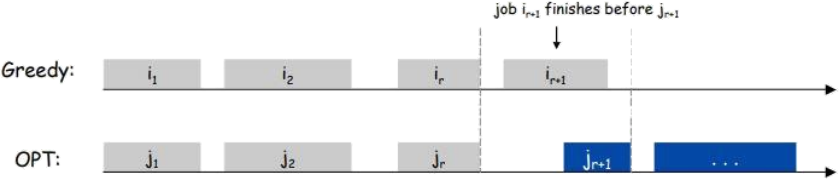
\includegraphics[width=0.67\linewidth]{figures/interval-scheduling-contradiction.png}
\end{center}

\subsubsection{By Induction}

\begin{listu}
    \item Let $S_j$ be the subset of jobs picked by greedy after considering the first $j$ jobs in the increasing order of finish time.

    Define $S_0 = \varnothing$.

    \item We call this partial solution \bred{promising} if there is a way to extend it to an optimal solution by picking some subset of jobs $j + 1, \dots, n$.

    $\exists T \subseteq \{j + 1, \dots, n\}$ such that $S_j \cup T$ is an optimal solution.

    \item \bred{Inductive claim:} for all $t \in \{0, 1, \dots, n\}$, $S_t$ is promising.

    \begin{listu}
        \item For $t = n$, if $S_n$ is promising, then it must be an optimal solution.

        \item We choose $t = 0$ as our base case since it is trivially promising.
    \end{listu}

    \item \textbf{Base case:} $t = 0$.

    For $t = 0$, $S_0 = \varnothing$ is promising. Any optimal solution extends it.

    \item \textbf{Inductive step:} $t - 1 \to t$.

    Suppose the claim holds for $t = j - 1$ and optimal solution $O_{j-1}$ extends $S_{j-1}$.

    At $t = j$, we have two cases:

    \begin{listo}
        \item Greedy did not select job $j$, so $S_j = S_{j-1}$.

        \begin{listu}
            \item Job $j$ must conflict with some job in $S_{j-1}$.
            \item Since $S_{j-1} \subseteq O_{j-1}$, $O_{j-1}$ also include pick job $j$.
            \item $O_j = O_{j-1}$ also extends $S_j = S_{j-1}$.
        \end{listu}

        \item Greedy selected job $j$, so $S_j = S_{j-1} \cup \{j\}$.

        \begin{listu}
            \item Consider the earliest job $r$ in $O_{j-1} \setminus S_{j-1}$.
            \item Consider $O_j$ contained by replacing $r$ with $j$ in $O_{j-1}$.
            \item Prove that $O_j$ is still feasible.
            \item $O_j$ extends $S_j$, as desired.
        \end{listu}

        \begin{center}
            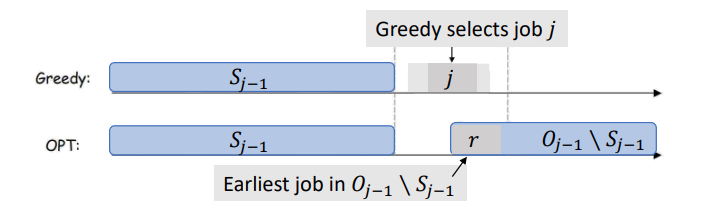
\includegraphics[width=0.67\linewidth]{figures/interval-scheduling-induction.png}
        \end{center}
    \end{listo}
\end{listu}

\subsubsection{Contradiction vs Induction}

Both methods make the same claim, that \begin{center}
    ``The greedy solution after $j$ iterations can be extended to an optimal solution, $\forall j$''.
\end{center} They also use the same key argument. \begin{center} \begin{minipage}[t]{0.9\linewidth}
    ``If the greedy solution after $j$ iterations can be extended to an optimal solution, then the greedy solution after $j + 1$ iterations can be extended to an optimal solution as well''
\end{minipage}
\end{center}

\begin{listu}
    \item For proof by induction, this is the key induction step.
    \item For proof by contradiction, we take the greatest $j$ for which the greedy solution can be extended to an optimal solution, and derive a contradiction by extending the greedy solution after $j + 1$ iterations.
\end{listu}

\section{Interval Partitioning}

\subsection{Problem Definition}

\begin{listu}
    \item Job $j$ starts at time $s_j$ and finishes at time $f_j$.
    \item Two jobs are compatible if they do not overlap.
    \item \textbf{Goal:} group jobs into fewest partitions such that jobs in the same partition are compatible.
\end{listu}

\begin{example}
    Think of scheduling lectures for various courses into as few classrooms as possible.

    This schedule uses \bred{4} classrooms for scheduling 10 lectures, but we can do better.

    \begin{center}
        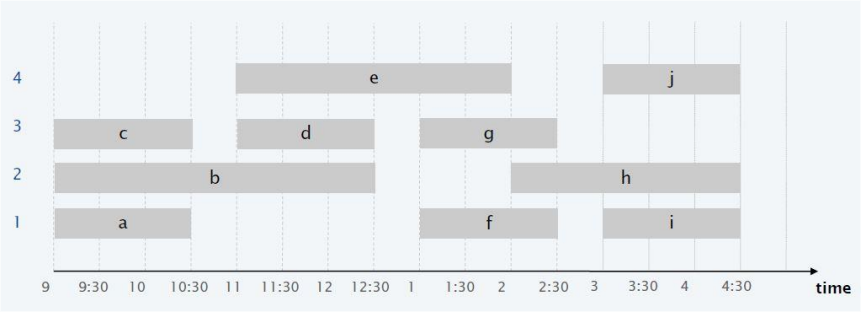
\includegraphics[width=0.55\linewidth]{figures/interval-scheduling-4-classrooms.png}
    \end{center}

    This schedule uses \bred{3} classrooms for scheduling 10 lectures, which is optimal.

    \begin{center}
        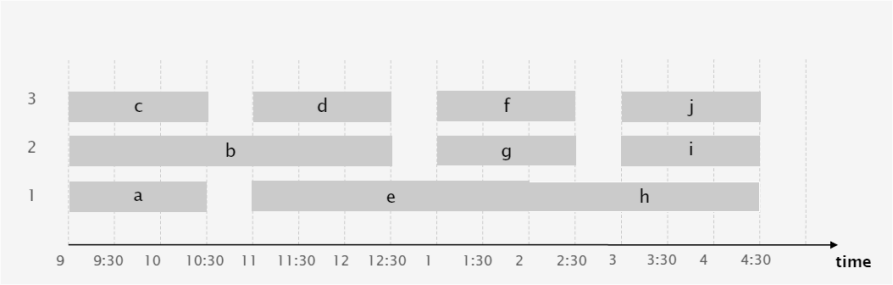
\includegraphics[width=0.55\linewidth]{figures/interval-scheduling-3-classrooms.png}
    \end{center}
\end{example}

One idea to solve this problem is to find the maximum compatible set using the previously greedy EFT algorithm, and then remove these jobs from the set and repeat. However, this is not optimal.

\subsection{Greedy Algorithm}

The greedy algorithm for interval partitioning follows the template

\begin{listu}
    \item Go through lectures in some ``natural'' order.
    \item Assign each lecture to an \itblue{arbitrary} compatible classroom, and create a new classroom if the lecture conflicts with every existing classroom
\end{listu}

If later we figures that arbitrary assignment is not optimal, we may need to go back to this template, and use a more careful assignment strategy.

\begin{minipage}[t]{0.6\linewidth}
    {~~~}

    It still makes sense to use the same ``natural'' orders as before: earliest start time, earliest finish time, shortest interval, and fewest conflicts.

    {~~~}

    Similar to interval scheduling, when we assign each lecture to an arbitrary compatible classroom, three of these heuristics do not work.
\end{minipage}
\hfil%
\begin{minipage}[t]{0.35\linewidth}
    \begin{center}
        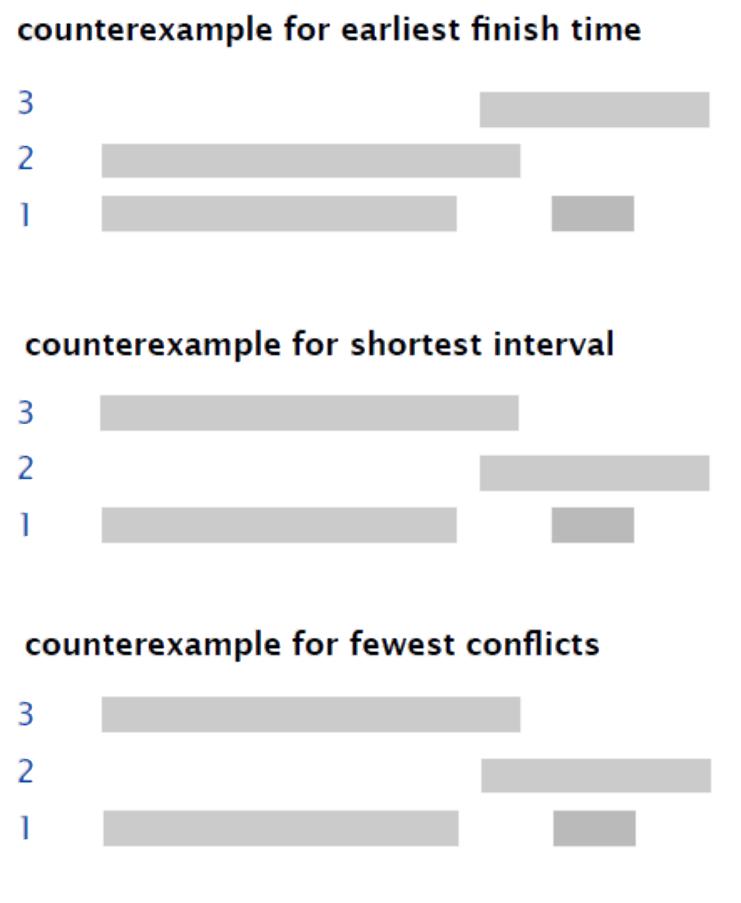
\includegraphics[width=0.9\linewidth,valign=t]{figures/interval-scheduling-counterexample.png}
    \end{center}
\end{minipage}

\begin{algorithm}
    \begin{algorithmic}
        \Function{Earliest-Start-Time-First}{$n, s_1, s_2, \dots, s_n, f_1, f_2, \dots, f_n$}
            \State \Call{Sort}{lectures} bt start time so that $s_1 \le s_2 \le \cdots \le s_n$
            \State $d \gets 0$
            \For{$i = 1$ \To $n$}
                \If{lecture $j$ is compatible with some classroom}
                    \State Schedule lecture $j$ in any such classroom $k$
                \Else
                    \State Allocate a new classroom $d + 1$
                    \State Schedule lecture $j$ in classroom $d + 1$
                    \State $d \gets d + 1$
                \EndIf
            \EndFor

            \State \Return schedule
        \EndFunction
    \end{algorithmic}
\end{algorithm}

\subsubsection{Running Time}

\begin{listu}
    \item \textbf{Key step:} checking if the next lecture can be scheduled at some classroom.

    \item We can tore classrooms in a priority queue, with the key being the latest finish time of any lecture in the classroom.

    \item Determining if lecture $j$ is compatible with some classrooms is equivalent to determining whether $s_j \ge f_k$ for some classroom $k$.

    \begin{listu}
        \item If it is compatible, we add jecture $j$ to classroom $k$ with minimum key, and increase its key to $f_j$.
        \item If it is not compatible, we add a new classroom to the priority queue with key $f_j$.
    \end{listu}

    \item There are $\mathcal{O}(n)$ priority queue operations, each of which takes $\mathcal{O}(\log n)$ time.

    This gives a total running time of \[
        \mathcal{O}(n \log n).
    \]
\end{listu}

\subsection{Proof of Optimality}

\subsubsection{Lower Bound}

The number of classrooms used by any algorithm is at least the number of lectures running at any time, which we call the ``depth''. This is because each classroom can only hold one lecture at a time.

We claim that the greedy algorithm uses only these many classrooms.

\begin{center}
    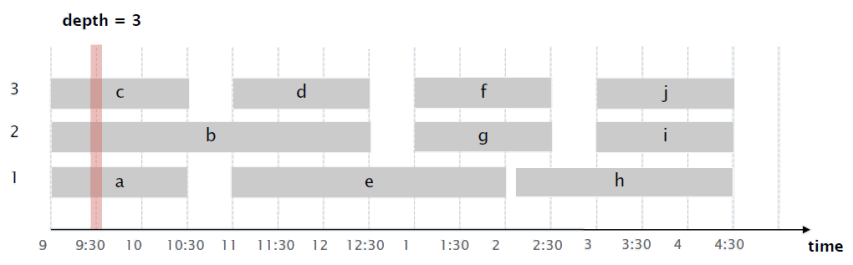
\includegraphics[width=0.75\linewidth]{figures/interval-scheduling-lower-bound.png}
\end{center}

\subsubsection{Upper Bound}

\begin{listu}
    \item Let $d$ be the number of classrooms used by the greedy algorithm.

    \item Classroom $d$ was opened because there was a lecture $j$ which was incompatible with some lectures already scheduled in each of $d - 1$ other classrooms.

    \item All these $d$ lectures end after $s_j$.

    Since we \itblue{have sorted the lectures by start time}, they all start at/before $s_j$.

    \item So, at time $s_j$, we have $d$ mutually overlapping lectures.

    \item Hence, $\text{depth} \ge d$, which is the number of classrooms used by the greedy algorithm.
\end{listu}

By the lower bound and the upper bound, we have that the greedy algorithm is optimal. \qed

\subsection{Interval Graphs}

\begin{definition}
    An \term{interval graph} is a graph whose vertices can be mapped to intervals on the real line such that two vertices are adjacent if and only if their corresponding intervals overlap.
\end{definition}

With this definition, we can restate the interval scheduling and partitioning problems as graph problems.
\begin{listu}
    \item Interval Scheduling: find a maximum independent set (MIS) in an interval graph.
    \item Interval Partitioning: find a minimum coloring of an interval graph.
\end{listu}

MIS and graph coloring are NP-hard for general graphs, but they are efficiently solvable for interval graphs.
\begin{listu}
    \item Graphs which can be obtained from incompatibility of intervals
    \item In fact, this holds even when we are not given an interval representation of the graph
\end{listu}

\section{Minimizing Lateness}

\subsection{Problem Definition}

\begin{listu}
    \item We have a single machine.
    \item Each job $j$ requires $t_j$ units of time and is due by time $d_j$.
    \item If it is scheduled to start at time $s_j$, then it finishes at time $f_j = s_j + t_j$.
    \item The \term{lateness} of job $j$ is defined as $\ell_j = \max\{0, f_j - d_j\}$.
    \item \textbf{Goal:} schedule jobs to minimize the maximum lateness, $L = \max_j \ell_j$.
\end{listu}

To contrast with interval scheduling problems, we now can decide the start time of each job, and the deadlines are soft.

\begin{example}
    Below are some jobs given to us.

    \begin{table}[ht!]
        \centering
        \begin{tabular}{c|c|c|c|c|c|c}
                  & 1 & 2 & 3 & 4 & 5  & 6  \\ \hline
            $t_j$ & 3 & 2 & 1 & 4 & 3  & 2  \\ \hline
            $d_j$ & 6 & 8 & 9 & 9 & 14 & 15 \\
        \end{tabular}
    \end{table}

    An example schedule would be
    \begin{center}
        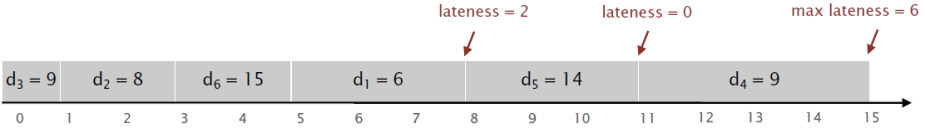
\includegraphics[width=0.8\linewidth]{figures/minimizing-lateness-example.png}
    \end{center}

    Note that this schedule is not optimal.
\end{example}

\subsection{Greedy Algorithm}

The greedy algorithm for minimizing lateness follows the template
\begin{listu}
    \item Consider jobs one-by-one in some ``natural'' order.
    \item Schedule jobs in this order (nothing special to do here, since we have to schedule all jobs and there is only one machine available)
\end{listu}

Here, the ``natural'' order may be
\begin{listu}
    \item \textbf{Shortest processing time first:} ascending order of processing time $t_j$.
    \item \textbf{Earliest deadline first:} ascending order of due time $d_j$.
    \item \textbf{Smallest slack first:} ascending order of $d_j - t_j$.
\end{listu}

As expected, some of these orders will not yield the optimal solution.

{~~~}

\begin{minipage}[t]{0.45\linewidth}
    \begin{center}
        Shortest processing time first

        \begin{tabular}{c|c|c}
                  & 1   & 2  \\ \hline
            $t_j$ & 1   & 10 \\ \hline
            $d_j$ & 100 & 10 \\
        \end{tabular}
    \end{center}
\end{minipage}
\hfil%
\begin{minipage}[t]{0.45\linewidth}
    \begin{center}
        Smallest slack first

        \begin{tabular}{c|c|c}
                  & 1 & 2  \\ \hline
            $t_j$ & 1 & 10 \\ \hline
            $d_j$ & 2 & 10 \\
        \end{tabular}
    \end{center}
\end{minipage}

{~~~}

{~~~}

We can implement the greedy algorithm using \bred{earliest deadline first}.

\begin{algorithm}
    \begin{algorithmic}
        \Function{Earliest-Deadline-First}{$n, t_1, t_2, \dots, t_n, d_1, d_2, \dots, d_n$}
            \State \Call{Sort}{jobs} by deadline so that $d_1 \le d_2 \le \cdots \le d_n$
            \State $t \gets 0$
            \For{$j = 1$ \To $n$}
                \State Assign job $j$ to interval $[t, t + t_j]$
                \State $s_j \gets t$, $f_j \gets t + t_j$
                \State $t \gets t + t_j$
            \EndFor

            \State \Return intervals $[s_1, f_1], [s_2, f_2], \dots, [s_n, f_n]$
        \EndFunction
    \end{algorithmic}
\end{algorithm}

\subsection{Proof of Optimality}

We make the following observations.

\begin{listu}
    \item \textbf{Observation 1:} There is an optimal schedule with \bred{no idle time}.

    \begin{center}
        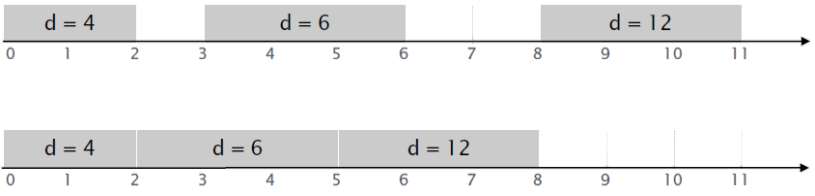
\includegraphics[width=0.67\linewidth]{figures/minimizing-lateness-observation-1.png}
    \end{center}

    \item \textbf{Observation 2:} Earliest deadline first has no idle time.

    \item \textbf{Observation 3:} By definition, earliest deadline first has no inversions.

    There, an inversion is a pair of jobs $i$ and $j$ such that $d_i < d_j$ but $j$ is scheduled before $i$.

    \item \textbf{Observation 4:} If a schedule with no idle time has at least one inversion, it has a pair of inverted jobs scheduled consecutively.

    \item \textbf{Observation 5:} Swapping adjacently scheduled inverted jobs does not increase lateness but reduces the number of inversions by one.

    \begin{center}
        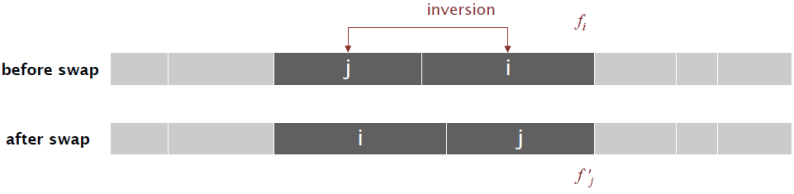
\includegraphics[width=0.67\linewidth]{figures/minimizing-lateness-observation-5.png}
    \end{center}

    \textit{Proof.}
        Let $\ell_k$ and $\ell'_k$ denote the lateness of job $k$ before and after the swap.

        Let $L = \max_k \ell_k$ and $L' = \max_k \ell'_k$ be the maximum lateness.

        Let $i$ and $j$ be the inverted jobs.

        \begin{listu}
            \item $\ell_k = \ell'_k$ for all $k \ne i, j$.

            \item $\ell'_i \le \ell_i$

            \item $\ell'j = f'_j - d_j = f_i - d_j \le f_i - d_i = \ell_i$

            This uses the fact that, due to the inversion, $d_j \ge d_i$.

            \item $\displaystyle L' = \max\left\{\ell'_i, \ell'_j, \max_{k \ne i, j} \ell'_k\right\} \le \max\left\{\ell_i, \ell_j, \max_{k \ne i, j} \ell_k\right\} = L$ \qed
        \end{listu}
\end{listu}

Observations 4 and 5 together is the key to the proof of optimality.

\begin{remark}
    Recall the proof of optimality of the greedy algorithm for interval scheduling

    \begin{listu}
        \item Take an optimal solution matching greedy for $r$ steps, and produced another optimal solution matching greedy for $r + 1$ steps
        \item ``Wrapped'' in a proof by contradiction or proof by induction
    \end{listu}

    Observations 4 and 5 provide a similar structure. If optimal solution does not fully match greedy (the number of inversions $\ge 1$), we can swap an adjacent inverted pair and reduce the number of inversions by one.
\end{remark}

\subsubsection{By Contradiction}

\begin{proof}
    Suppose for contradiction that the greedy EDF solution is not optimal

    \begin{listu}
        \item Consider an optimal schedule $S^*$ with the fewest inversions\footnote{Note that this part is a little flawed, as $S^*$ may be different from the greedy EDF solution based on how we break ties. To fix this, we can simply change the way we break ties until we get the same solution as the greedy EDF solution. Since these jobs are adjacent, we can do this by swapping adjacent jobs, and, by Observation 5, this will not increase the lateness, so the solution remains optimal.}. Without loss of generality, assume it has no idle time.

        \item Since the greedy EDF solution is not optimal, there is at least one inversion in $S^*$.

        \item By Observation 4, the pair of inversion $(i, j)$ are scheduled consecutively (adjacent).

        \item By Observation 5, swapping the adjacent pair keeps the schedule optimal but reduces the number of inversions by 1

        This is a contradiction, as $S^*$ has the fewest inversions.
    \end{listu}

    Thus, the greedy EDF solution is optimal.
\end{proof}

\subsubsection{By Induction}

\begin{proof}
    By induction on the number of inversions in an optimal schedule.

    \begin{claim}
        For each $r \in \left\{ 0, 1, 2, \dots, \binom{n}{2} \right\}$, there is an optimal schedule with at most $r$ inversions.
    \end{claim}

    \begin{listu}
        \item \textbf{Base case:} $r = \binom{n}{2}$

        This is trivially true.

        \item \textbf{Inductive step:} $t + 1 \to t$

        Suppose the claim holds for $t + 1$.

        Take an optimal schedule $S^*$ with at most $t + 1$ inversions.

        Without loss of generality, assume it has no idle time.

        \begin{listu}
            \item If $S^*$ has at most $t$ inversions, we are done.

            \item If $S^*$ has exactly $t + 1$ inversions, then there is a pair of inverted jobs $(i, j)$ scheduled consecutively by Observation 4.

            By Observation 5, swapping the adjacent pair keeps the schedule optimal but reduces the number of inversions by 1.

            The number of inversions in the new schedule is at most $t$, and the claim holds.
        \end{listu}
    \end{listu}

    Claim for $r = 0$ shows optimality of the greedy EDF solution.
\end{proof}

\subsubsection{Contradiction vs Induction}

The favour over contradiction or induction is a matter of taste. It may be the case that for some problems, one method is easier to apply than the other. There is no inherent difference in the two methods, as they both make the same claim and use the same key argument, and one does not need to stick to one method. Meanwhile, as we have seen for the interval partitioning problem, sometimes we may require an entirely different method to prove optimality.
\section{Lossless Compression}

\subsection{Problem Definition}

\begin{example}
    We have a document that is written using $n$ distinct labels. The na\"ive encoding would use $\log_2 n$ bits for each label, but it is not optimal. We can assign shorter encodings to more frequent labels.

    {~~~}

    Say we assign $a = 0$, $b = 1$, $c = 01$, $\dots$ based on the frequency of the labels. However, now we have created confusion when decoding, as $01$ can be decoded as either `ab' or `c'.

    {~~~}

    To avoid conflicts, we need a \term{prefix-free encoding}, where no label is a prefix of another label. Now, we can read left to right, and whenever the part to the left becomes a valid encoding, we greedily decode it, and continue with the rest.
\end{example}

\begin{definition}[Lossless Compression]\index{Lossless Compression}\label{def:lossless-compression}
    Given $n$ symbols and their frequencies $(w_1, \dots, w_n)$, find a prefix-tree encoding with length $(\ell_1, \dots, \ell_n)$ assigned to the symbols which minimizes $\displaystyle \sum_{i=1}^n w_i \ell_i$.
\end{definition}

We observe that prefix-free encodings can be represented by a binary tree.

\begin{center}
    \tikzsetnextfilename{huffman}
    \tikzexternalenable
    \begin{tikzpicture}[
        inte-node/.style={circle,text=white,fill=orange},
        leaf-node/.style={rectangle,text=white,fill=orange},
        baseline=(current bounding box.north)
    ]
        \node[inte-node] (100) at (0, 0) {$100$};

        \node[leaf-node] (a)  at (-3, -0.75) {$a:42$};
        \node[inte-node] (58) at (3, -0.75) {$58$};

        \node[inte-node] (23) at (1, -1.5) {$23$};
        \node[inte-node] (35) at (5, -1.5) {$35$};

        \node[leaf-node] (e)  at (0, -2.25) {$e:11$};
        \node[leaf-node] (f)  at (2, -2.25) {$f:12$};
        \node[inte-node] (15) at (4, -2.25) {$15$};
        \node[leaf-node] (b)  at (6, -2.25) {$b:20$};

        \node[leaf-node] (c)  at (3.25, -3) {$c:5$};
        \node[leaf-node] (d)  at (4.75, -3) {$d:10$};

        \draw[thick] (100) -- (a) node[midway, above left] {0};
        \draw[thick] (100) -- (58) node[midway, above right] {1};
        \draw[thick] (58) -- (23) node[midway, above left] {0};
        \draw[thick] (58) -- (35) node[midway, above right] {1};
        \draw[thick] (23) -- (e) node[midway, above left] {0};
        \draw[thick] (23) -- (f) node[midway, above right] {1};
        \draw[thick] (35) -- (15) node[midway, above left] {0};
        \draw[thick] (35) -- (b) node[midway, above right] {1};
        \draw[thick] (15) -- (c) node[midway, above left] {0};
        \draw[thick] (15) -- (d) node[midway, above right] {1};
    \end{tikzpicture}
    \tikzexternaldisable
\end{center}

\vspace{-3em}
\subsection{Huffman Encoding}

The Huffman encoding algorithm is a greedy algorithm that generates an optimal prefix-tree encoding for a given set of symbols and their frequencies. 

% \vspace{-1em}
\begin{algorithm}
    \begin{algorithmic}
        \Function{Huffman-Encoding}{$n, w_1, w_2, \dots, w_n$}
            \State $Q \gets \text{Priority-Queue}$
            \For{each symbol $x$}
                \State \Call{Insert}{$Q, x, w_x$}
            \EndFor

            \For{$i = 1$ \To $n - 1$}
                \State $(x, w_x) \gets \text{Extract-Min}(Q)$
                \State $(y, w_y) \gets \text{Extract-Min}(Q)$
                \State \Call{Insert}{$Q, (x, y), w_x + w_y$}
            \EndFor

            \State \Return the root of the tree
        \EndFunction
    \end{algorithmic}
\end{algorithm}

\newpage
\begin{example}
    We use the Huffman encoding algorithm to generate the tree for the previous example.

    \begin{center}
        \tikzexternalenable
        \begin{tikzpicture}[
            inte-node/.style={circle,text=white,fill=orange},
            leaf-node/.style={rectangle,text=white,fill=orange},
        ]
            \node[leaf-node] (c) at (-5, 0) {$c:5$};
            \node[leaf-node] (d) at (-3, 0) {$d:10$};
            \node[leaf-node] (e) at (-1, 0) {$e:11$};
            \node[leaf-node] (f) at (1, 0) {$f:12$};
            \node[leaf-node] (b) at (3, 0) {$b:20$};
            \node[leaf-node] (a) at (5, 0) {$a:42$};
        \end{tikzpicture}
        \tikzexternaldisable

        \vspace{0.25em} 
\includegraphics[width=2em]{tikz/down-arrow.pdf} \vspace{0.25em}

        \tikzexternalenable
        \begin{tikzpicture}[
            inte-node/.style={circle,text=white,fill=orange},
            leaf-node/.style={rectangle,text=white,fill=orange},
        ]
            \node[leaf-node] (e) at (-4, 0) {$e:11$};
            \node[leaf-node] (f) at (-2, 0) {$f:12$};
            \node[leaf-node] (b) at (2, 0) {$b:20$};
            \node[leaf-node] (a) at (4, 0) {$a:42$};

            \node[inte-node] (15) at (0, 0) {$15$};
            \node[leaf-node] (c) at (-1, -0.75) {$c:5$};
            \node[leaf-node] (d) at (1, -0.75) {$d:10$};

            \draw[thick] (15) -- (c);
            \draw[thick] (15) -- (d);
        \end{tikzpicture}
        \tikzexternaldisable

        \vspace{0.25em} 
\includegraphics[width=2em]{tikz/down-arrow.pdf} \vspace{0.25em}

        \tikzexternalenable
        \begin{tikzpicture}[
            inte-node/.style={circle,text=white,fill=orange},
            leaf-node/.style={rectangle,text=white,fill=orange},
        ]
            \node[leaf-node] (b) at (-1, 0) {$b:20$};
            \node[leaf-node] (a) at (3, 0) {$a:42$};

            \node[inte-node] (15) at (-3, 0) {$15$};
            \node[leaf-node] (c) at (-4, -0.75) {$c:5$};
            \node[leaf-node] (d) at (-2, -0.75) {$d:10$};

            \node[inte-node] (23) at (1, 0) {$23$};
            \node[leaf-node] (e) at (0, -0.75) {$e:11$};
            \node[leaf-node] (f) at (2, -0.75) {$f:12$};

            \draw[thick] (15) -- (c);
            \draw[thick] (15) -- (d);
            \draw[thick] (23) -- (e);
            \draw[thick] (23) -- (f);
        \end{tikzpicture}
        \tikzexternaldisable

        \vspace{0.25em} 
\includegraphics[width=2em]{tikz/down-arrow.pdf} \vspace{0.25em}

        \tikzexternalenable
        \begin{tikzpicture}[
            inte-node/.style={circle,text=white,fill=orange},
            leaf-node/.style={rectangle,text=white,fill=orange},
        ]
            \node[leaf-node] (a) at (4, 0) {$a:42$};
            
            \node[inte-node] (23) at (-3, 0) {$23$};
            \node[leaf-node] (e) at (-4, -0.75) {$e:11$};
            \node[leaf-node] (f) at (-2, -0.75) {$f:12$};

            \node[inte-node] (35) at (1, 0) {$35$};
            \node[inte-node] (15) at (0, -0.75) {$15$};
            \node[leaf-node] (c) at (-1, -1.5) {$c:5$};
            \node[leaf-node] (d) at (1, -1.5) {$d:10$};
            \node[leaf-node] (b) at (2, -0.75) {$b:20$};

            \draw[thick] (15) -- (c);
            \draw[thick] (15) -- (d);
            \draw[thick] (23) -- (e);
            \draw[thick] (23) -- (f);
            \draw[thick] (35) -- (15);
            \draw[thick] (35) -- (b);
        \end{tikzpicture}
        \tikzexternaldisable

        \vspace{0.25em} 
\includegraphics[width=2em]{tikz/down-arrow.pdf} \vspace{0.25em}

        \tikzexternalenable
        \begin{tikzpicture}[
            inte-node/.style={circle,text=white,fill=orange},
            leaf-node/.style={rectangle,text=white,fill=orange},
        ]
            \node[leaf-node] (a) at (-2.5, 0) {$a:42$};

            \node[inte-node] (58) at (0, 0) {$58$};

            \node[inte-node] (23) at (-2, -0.75) {$23$};
            \node[leaf-node] (e) at (-3, -1.5) {$e:11$};
            \node[leaf-node] (f) at (-1, -1.5) {$f:12$};

            \node[inte-node] (35) at (2, -0.75) {$35$};
            \node[inte-node] (15) at (1, -1.5) {$15$};
            \node[leaf-node] (c) at (0, -2.25) {$c:5$};
            \node[leaf-node] (d) at (2, -2.25) {$d:10$};
            \node[leaf-node] (b) at (3, -1.5) {$b:20$};

            \draw[thick] (15) -- (c);
            \draw[thick] (15) -- (d);
            \draw[thick] (23) -- (e);
            \draw[thick] (23) -- (f);
            \draw[thick] (35) -- (15);
            \draw[thick] (35) -- (b);
            \draw[thick] (58) -- (23);
            \draw[thick] (58) -- (35);
        \end{tikzpicture}

        \vspace{0.25em} 
\includegraphics[width=2em]{tikz/down-arrow.pdf} \vspace{0.25em}

        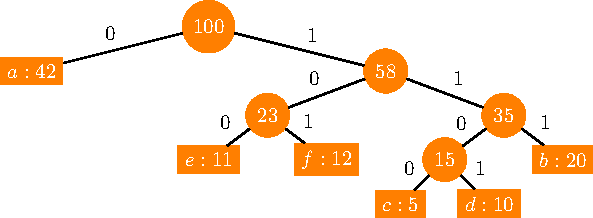
\includegraphics{tikz/huffman.pdf}
    \end{center}
\end{example}

\subsubsection{Running Time}

The running time of the Huffman encoding algorithm is $\mathcal{O}(n \log n)$. However, it can be made $\bigo{n}$ if the labels are sorted by frequency, by using two queues. 

\subsection{Proof of Optimality}

\begin{proof}
    By induction on the number of symbols $n$.

    \begin{listu}
        \item \textbf{Base case:} $n = 2$

        Both encodings which assign 1 bit to each symbol are optimal.

        \item \textbf{Inductive step:} $n - 1 \to n$

        Assume Huffman encoding returns an optimal encoding with $n - 1$ symbols. Consider the case with $n$ symbols.

        \begin{lemma*}[1]\label{lem:huffman-1}
            If $w_x < w_y$, then $\ell_x \ge \ell_y$ in any optimal tree.
        \end{lemma*}

        \begin{proof}
            Proof of \hyperref[lem:huffman-1]{Lemma 1}

            Suppose for contradiction that $w_x < w_y$ and $\ell_x < \ell_y$ in an optimal tree.

            Swapping $x$ and $y$ strictly decreases the total encoding length, as \[
                w_x \cdot \ell_y + w_y \cdot \ell_x < w_x \cdot \ell_x + w_y \cdot \ell_y.
            \]

            This is a contradiction.
        \end{proof}

        Consider the two symbols $x$ and $y$ with lowest frequency which Huffman encoding combines in the first step.

        \begin{lemma*}[2]\label{lem:huffman-2}
            Exists an optimal tree $T$ in which $x$ and $y$ are siblings.

            That is, for some $p$, $x$ and $y$ are assigned encodings of the form $p0$ and $p1$.
        \end{lemma*}

        \textit{Proof.}
            Proof of \hyperref[lem:huffman-2]{Lemma 2}

            \begin{listo}
                \item Let $T$ be an optimal tree.
                \item Let $x$ be the label with the lowest frequency in $T$.
                \item If $x$ does not have the longest encoding in $T$, swap it with the label with the longest encoding.
                \item Due to optimality, $x$ must have a sibling $y'$ (otherwise, we can swap $x$ with its parent and reduce the total encoding length).
                \item If $y'$ is not $y$, swap it with $y$.
                \item We check that Steps 3 and 5 does not change the overall length. \qed
            \end{listo}

        Let $x$ and $y$ be the two least frequency symbols that Huffman combines in the first step into ``$xy$''.

        Let $H$ be the Huffman tree produced. 

        Let $T$ be an optimal tree in which $x$ and $y$ are siblings.

        Let $H'$ and $T'$ be obtained from $H$ and $T$ bt treating $xy$ as one symbol with frequency $w_x + w_y$.

        By the inductive hypothesis, $T'$ is optimal for the $n - 1$ symbols, so $\textsc{Length}(H') \le \textsc{Length}(T')$.

        \begin{listu}
            \item $\textsc{Length}(H) = \textsc{Length}(H') + (w_x + w_y) \cdot 1$
            \item $\textsc{Length}(T) = \textsc{Length}(T') + (w_x + w_y) \cdot 1$
        \end{listu}

        Therefore, $\textsc{Length}(H) \le \textsc{Length}(T)$.
    \end{listu}

    Thus, the Huffman encoding algorithm returns an optimal encoding.
\end{proof}

\section{Other Greedy Algorithms}

\subsection{Dijkstra's Algorithm}\label{subsec:dijkstras-algorithm}

Dijsktra's algorithm is a greedy algorithm that finds the \itblue{shortest path} from a single source to all other vertices in a weighted graph. 

\begin{algorithm}[ht!]
    \begin{algorithmic}[1]
        \Function{Dijkstra}{$G, s$}
            \State $d[v] \gets \infty$ for all $v \in V$
            \State $d[s] \gets 0$
            \State $Q \gets \text{Priority-Queue}$
            \State \Call{Insert}{$Q, s, 0$}
            \While{$Q$ is not empty}
                \State $(u, d_u) \gets \text{Extract-Min}(Q)$
                \For{each edge $(u, v)$}
                    \If{$d_u + w(u, v) < d[v]$}
                        \State $d[v] \gets d_u + w(u, v)$
                        \State \Call{Insert}{$Q, v, d[v]$}
                    \EndIf
                \EndFor
            \EndWhile
            \State \Return $d$
        \EndFunction
    \end{algorithmic}
\end{algorithm}

\subsection{Kruskal's Algorithm and Prim's Algorithm}

Kruskal's algorithm and Prim's algorithm are greedy algorithms that finds a \itblue{minimum spanning tree} for a connected, undirected graph. 

% TODO